\section{Data preparation}\label{Data preparation}

In this paper data preparation for use in \gls{ai} model creation consists of two steps: acquisition and preprocessing.

\subsection{Acquisition}\label{Acquisition}

The data chosen for this study was a set of \gls{cpi}-deflated \gls{eer} obtained from the website of the \gls{ecb} \cite{forex-data}. The data consists of three sets of deflated \gls{eer} one on the basis of a group of 13 currencies, one 18 currencies and one 41 currencies. The data is sampled at a monthly frequency and covers the time frame from the 31.01.1993 to 31.10.2025. The currencies included in the dataset are: \gls{aed}, \gls{ars}, \gls{aud}, \gls{bgn}, \gls{brl}, \gls{cad}, \gls{chf}, \gls{clp}, \gls{cny}, \gls{cop}, \gls{czk}, \gls{dkk}, \gls{dzd}, \gls{eur}, \gls{gbp}, \gls{hkd}, \gls{huf}, \gls{idr}, \gls{ils}, \gls{inr}, \gls{isk}, \gls{jpy}, \gls{krw}, \gls{mad}, \gls{mxn}, \gls{myr}, \gls{nok}, \gls{nzd}, \gls{pen}, \gls{php}, \gls{pln}, \gls{ron}, \gls{rub}, \gls{sar}, \gls{sek}, \gls{sgd}, \gls{thb}, \gls{try}, \gls{twd}, \gls{uah}, \gls{usd}, \gls{zar}.

\subsection{Required preprocessing steps}\label{Required preprocessing steps}

The cleaning and preparation of the data was conducted in order to increase the accuracy of predictions as well as improve the efficiency of model training.

\subsubsection{Handling of missing values}\label{Handling of missing values}

The handling of missing values consisted of the removal of variables with more than two sequential variable specific missing values, caused by insufficient market activity and reporting inconsistencies, of which there was 1 (41-RUB), leaving behind 73 currency exchange rates. This step was crucial, as missing data can lead to biased estimates and can negatively affect the overall performance of predictive models \cite{techniques,rf-svr}.

\subsection{Optional intermediary steps}\label{Optional intermediary steps}

\subsubsection{Log transformation}\label{Log transformation}

In this step a natural logarithm transformation of the data was applied in order to stabilize the variance and prevent heteroscedacity \cite{nn-vs-chaotic,robust-regression,gbp-usd-forecasting}.

\subsubsection{Differencing}\label{Differencing}

In this step first-order differencing was applied to the dataset. This procedure causes the replacement of successive values with successive variations. This is a necessary step in the preparation of the data enabling the removal of trends, seasonality, and other non-stationary components from the original time series \cite{nn-vs-chaotic,robust-regression,gbp-usd-forecasting}.

\begin{figure}[h!]
    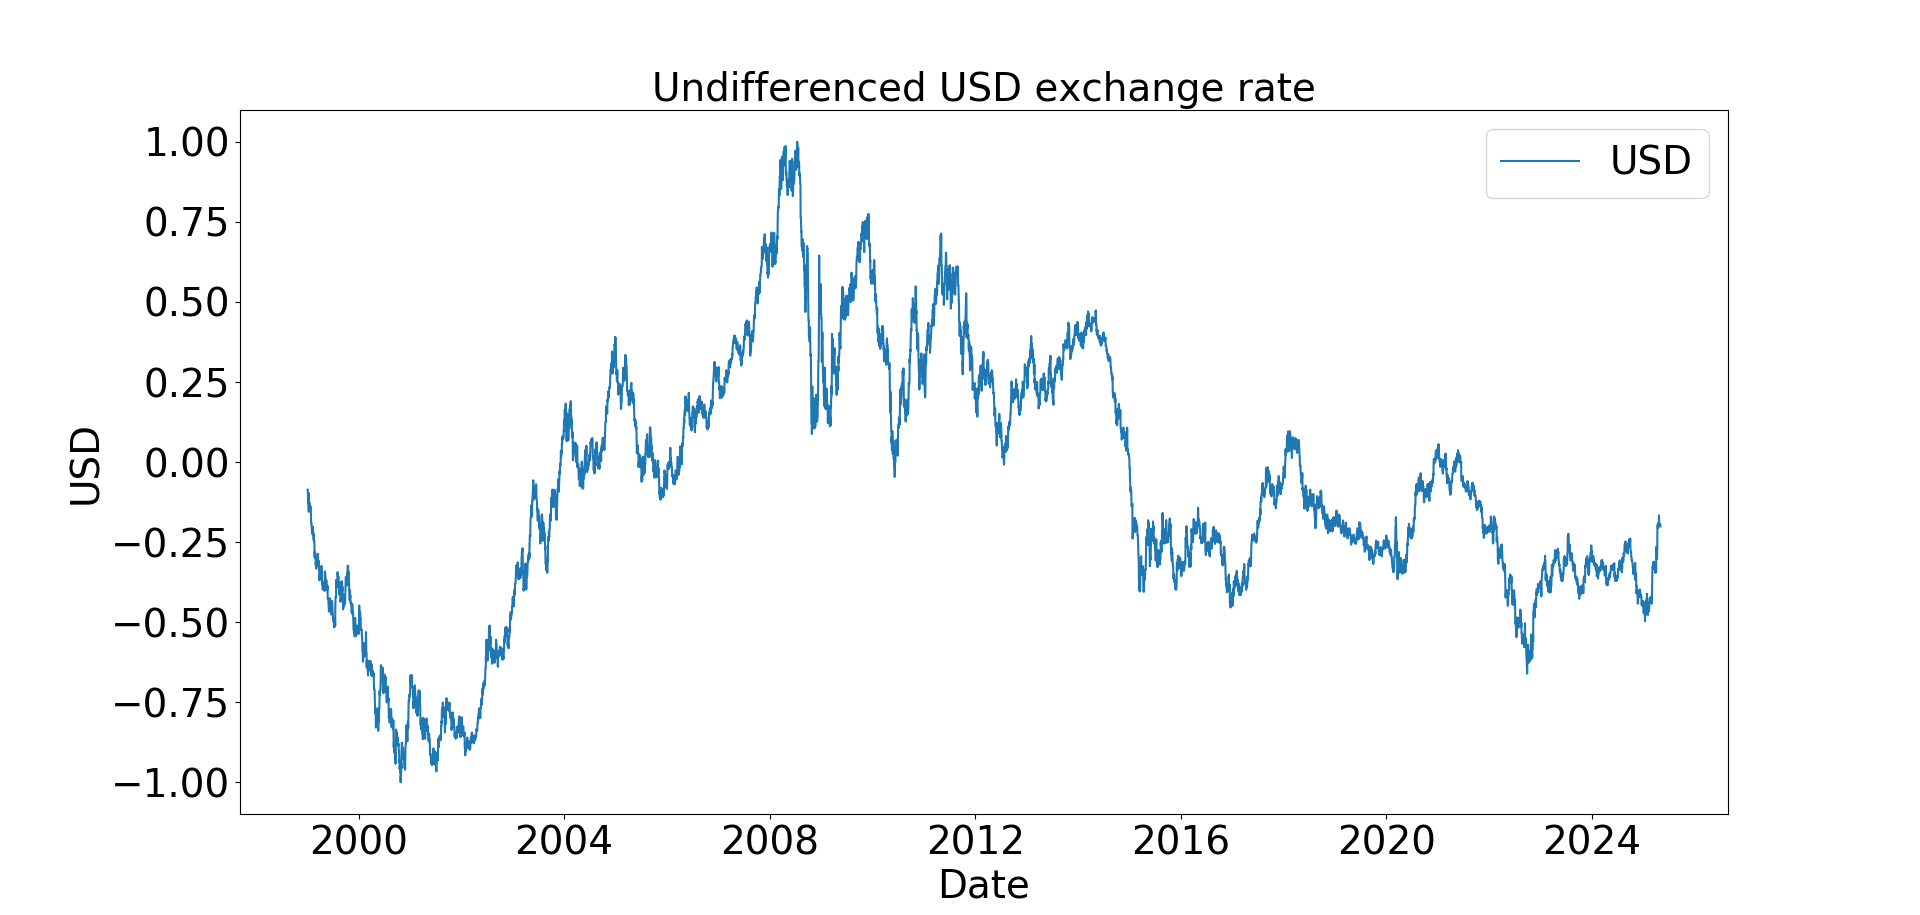
\includegraphics[width=\textwidth]{images/preprocessing/3-optional/differencing/usd-undiff.png}
    \centering
    \caption{The undifferenced forward filled \gls{usd} spot exchange rate.}
    \label{fig:usd-undiff}
\end{figure}

\begin{figure}[h!]
    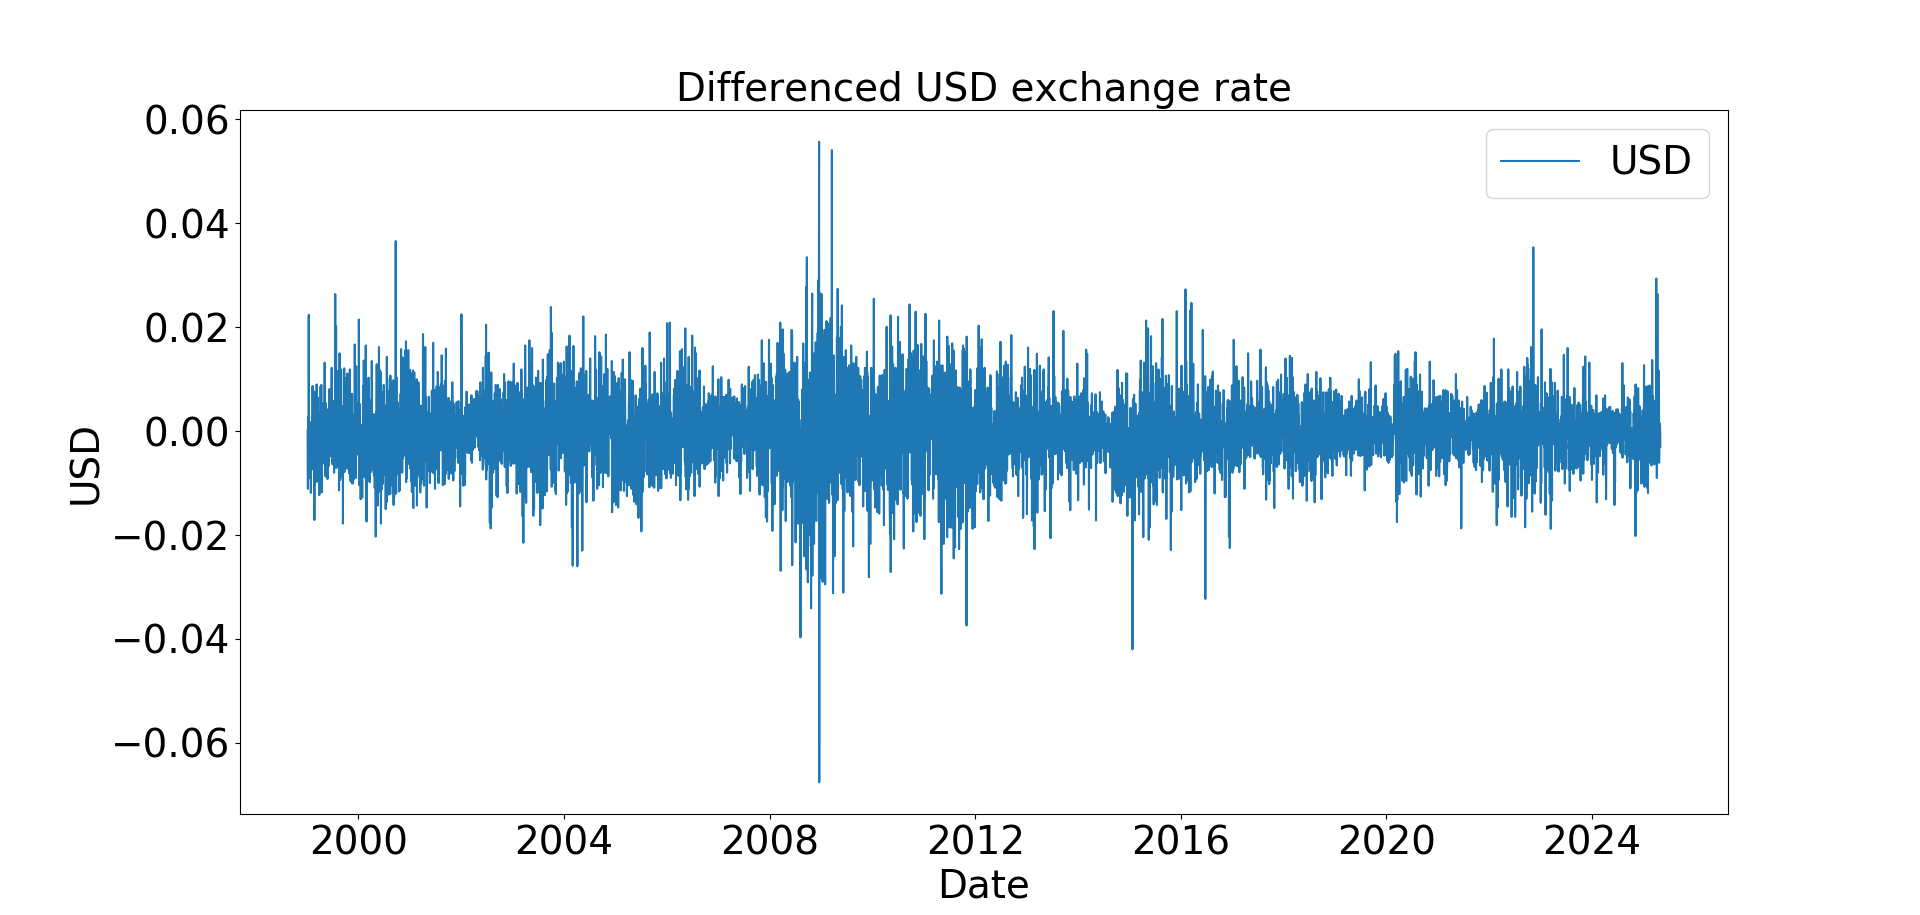
\includegraphics[width=\textwidth]{images/preprocessing/3-optional/differencing/usd-diff.png}
    \centering
    \caption{The differenced \gls{usd} spot exchange rate.}
    \label{fig:usd-diff}
\end{figure}

\subsubsection{Feature scaling}\label{Feature scaling}

Feature scaling is an essential step in the data preparation for many \gls{ai} models which often exhibit better training efficiency and forecasting accuracy with scaled data. This is especially true for \gls{mlp} and \gls{svr}. For the \gls{rf} machine learning model this step is not required due to insensitivity and as a result has been omitted. Two feature scaling methods where used in the data preparation process for different models in this paper. An visual representation of the effects of both can be seen in figure \ref{fig:usd-scaling}.

\begin{itemize}
    \item Normalization via scikit-learn's MinMaxScaler \cite{scikit-learn} to the range [-1,1] was used in the preparation of data primarily for use with the \gls{mlp} with the \gls{tanh} activation function \cite{nn-vs-chaotic,ann-2}.
    \item Standardization via scikit-learn's StandardScaler \cite{scikit-learn} to a mean of zero and a variance of one was used primarily in the data preparation pipeline for use with \gls{svr} \cite{genetic,rf-svr}.
\end{itemize}

\begin{figure}[h!]
    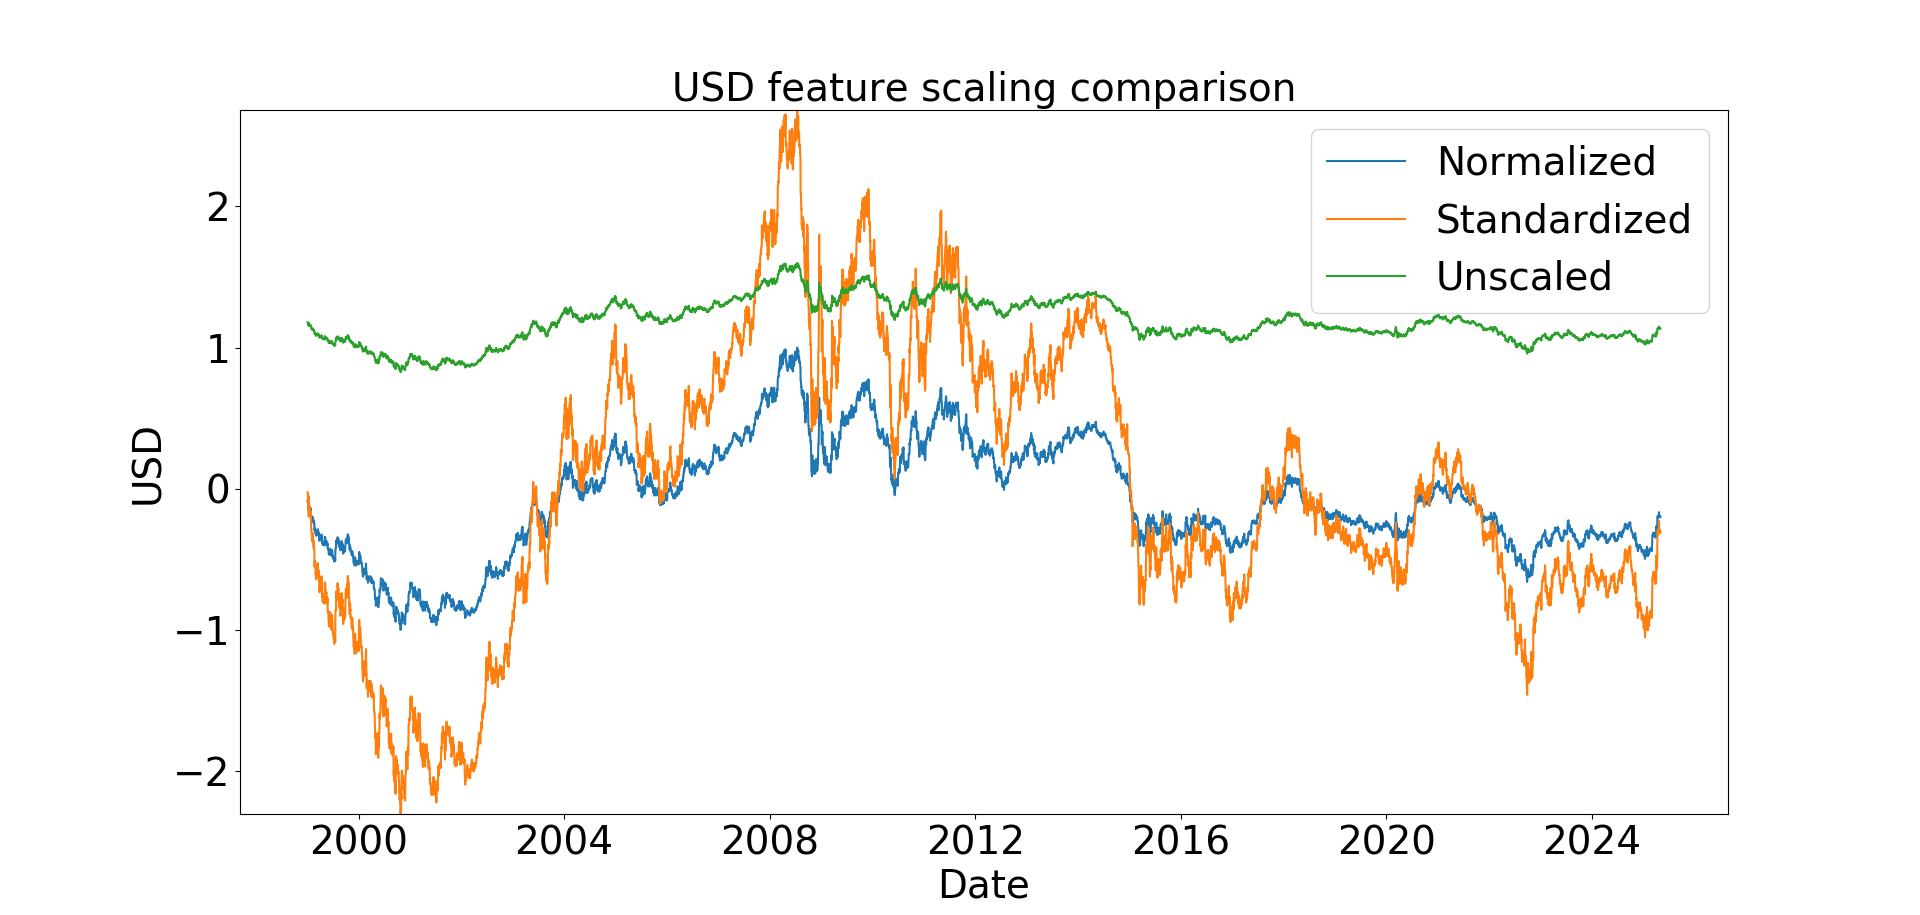
\includegraphics[width=\textwidth]{images/preprocessing/3-optional/scaling/usd-scaling.png}
    \centering
    \caption{A graphical comparison of normalization and standardization on the basis of the \gls{usd} spot exchange rate.}
    \label{fig:usd-scaling}
\end{figure}

\subsection{Required postprocessing steps}\label{Required postprocessing steps}

\subsubsection{Feature extraction}\label{Feature extraction}

For this step three different target variables were chosen each representing the \gls{usd} exchange rate for the different sized groupings of trading partners used for CPI-deflation. Time lagged versions of each dataset for each feature variable upto 12 months were created for each preprocessing variation \cite{rf-svr,gold}. An example of the shifting procedure for the \gls{usd} exchange rate is shown in figure \ref{fig:feature-extraction}.

\begin{figure}[h]
    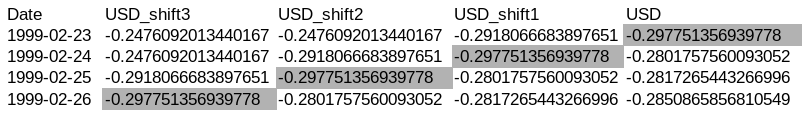
\includegraphics[width=\textwidth]{images/preprocessing/4-usd-shifts-3.png}
    \centering
    \caption{An example of a series of time shifts upto three days for the \gls{usd} exchange rate.}
    \label{fig:feature-extraction}
\end{figure}

% \subsubsection{Variable selection}\label{Variable selection}
% 
% In the next step scikit-learn's \gls{rfecv} \cite{scikit-learn} was used with the \gls{svr} model with a linear kernel as the estimator for feature importance ranking and optimal feature subset selection.
% 
% The \gls{cv} results for each dataset are presented in figure \ref{fig:rfecv}. As can be see the absence of scaling as well as in the case of scaling the chosen scaling methodology greatly affect the results of \gls{rfecv}.
% 
% For the \gls{mlp} dataset for which normalization was employed the optimal number of features selected by the \gls{rfecv} was 33.
% 
% For the \gls{svr} dataset for which standardization was employed the optimal number of features selected by the \gls{rfecv} was 9.
% 
% For the \gls{rf} dataset for which no scaling procedures were used the number of features selected by the \gls{rfecv} was 34.
% 
% \begin{figure}[h]
%     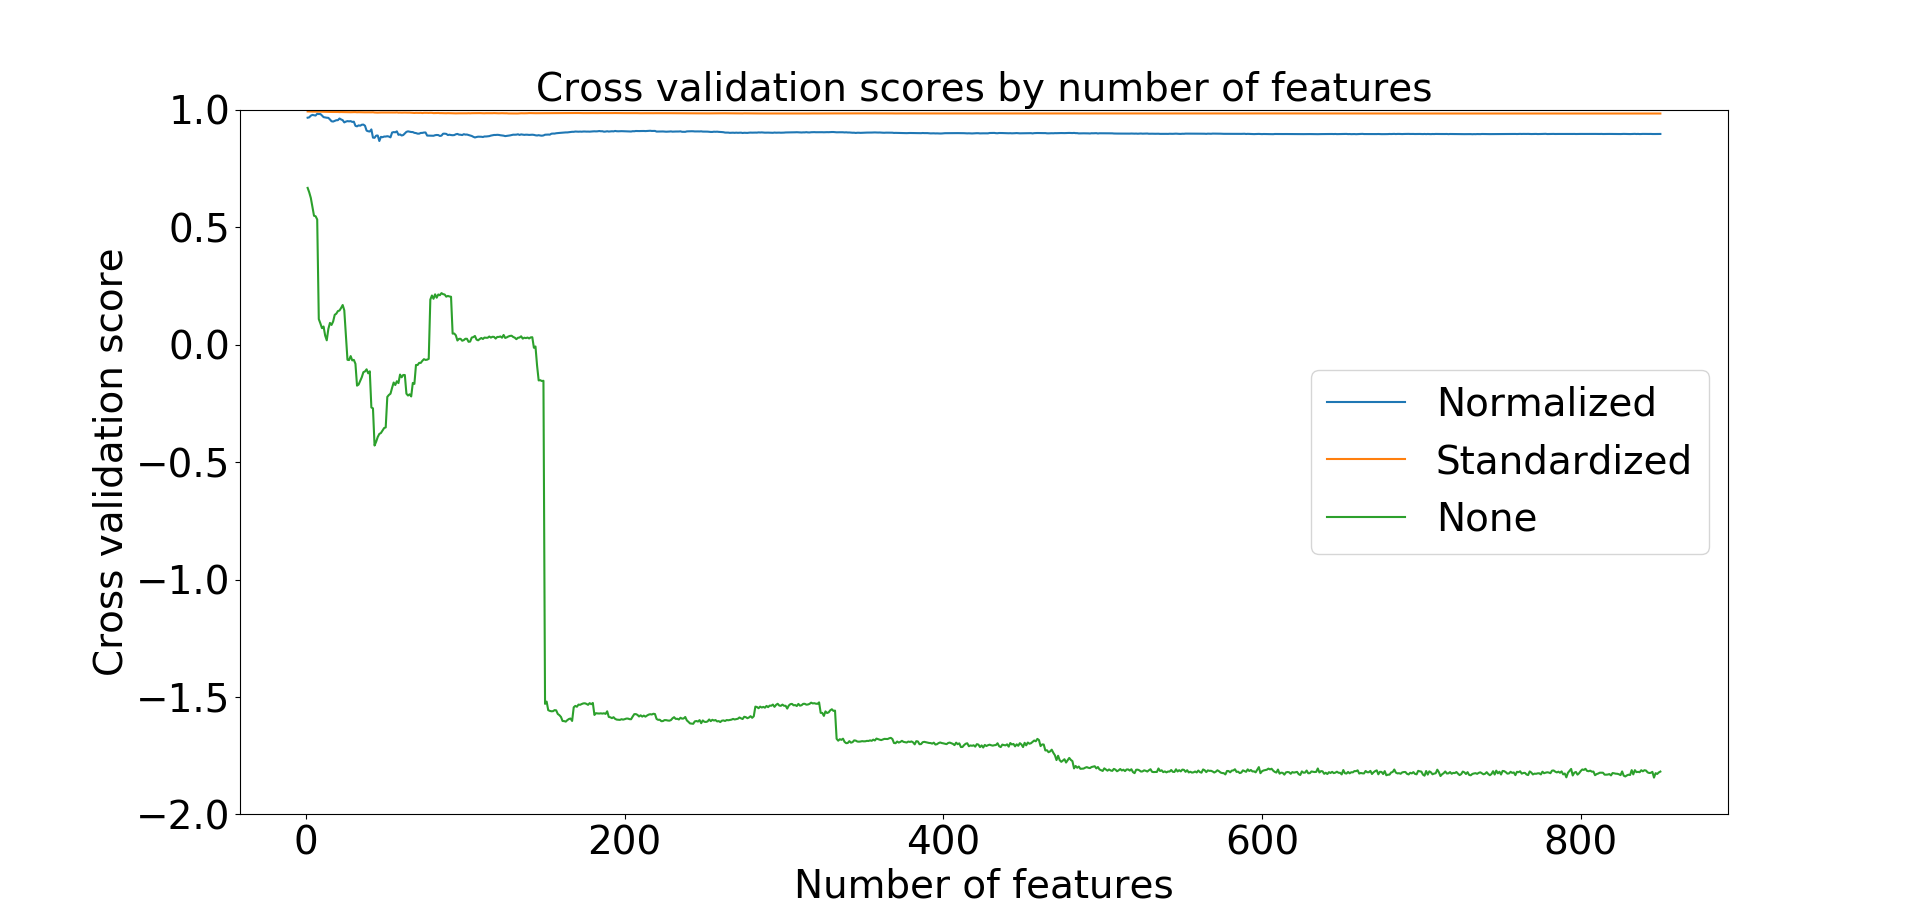
\includegraphics[width=\textwidth]{images/preprocessing/5-variable-selection/rfecv.png}
%     \centering
%     \caption{\Gls{cv} scores by number of features for normalized (\gls{mlp}), standardized (\gls{svr}) and unscaled (\gls{rf}) datasets.}
%     \label{fig:rfecv}
% \end{figure}

\subsubsection{Feature decorrelation}\label{Feature decorrelation}

In the next step a Pearson correlation matrix was constructed for the feature and target exchange rates to assess the linear relationships among them. Features exhibiting weak correlation $\le 0.1$ with the target were removed first, as they contribute noise without predictive signal. Next feature variables that had a high mutual correlation $\ge 0.9$ with at least one other feature were removed. This was done to mitigate the risk of multicollinearity, which can lead to the occurrence of amplifying or distorting effects during model training \cite{genetic}. As a result of this analysis, the initial feature set for each dataset processing variation was significantly reduced.

\subsubsection{Data split}\label{Data split}

For the purpose of model training and forecasting accuracy evaluation each dataset was split into two subsets with a separation strip equal to the degree of generated time lags (150) in order to prevent information leakage from the training set to the test set:
\begin{itemize}
    \item training $+$ validation (70\%) - for model training and k-fold cross-validation.
    \item testing (30\%) - for the final evaluation of the selected model in order to prevent overfitting and enable a unbiased evaluation of the model on new unseen data.
\end{itemize}

